
\documentclass{article} % For LaTeX2e
\usepackage{iclr2021_conference,times}

% Optional math commands from https://github.com/goodfeli/dlbook_notation.
% \input{math_commands.tex}

\usepackage[utf8]{inputenc}
\usepackage[english]{babel}
\usepackage{graphicx, color}
\usepackage[a4paper,margin=2cm]{geometry}
\usepackage{hyperref}
% \usepackage[numbers]{natbib}
\usepackage{subfiles}
% \usepackage{refcheck}
\usepackage{csquotes}
\usepackage{titlesec}
\usepackage{textcomp}  % \textquotesingle
% \usepackage{fontspec}
% \setmainfont{Symbola}
\usepackage{siunitx}
\sisetup{output-exponent-marker=\ensuremath{\mathrm{e}}}
% \usepackage{dirtytalk}
\usepackage{epigraph}
\usepackage{amsfonts}
\usepackage{algorithm}
\usepackage{algpseudocode}
\usepackage{mathtools}
% \usepackage{url}


\title{Type-driven Neural Programming by Example}

% Authors must not appear in the submitted version. They should be hidden
% as long as the \iclrfinalcopy macro remains commented out below.
% Non-anonymous submissions will be rejected without review.

\author{
   Kiara Grouwstra
   % \thanks{ Use footnote for providing further information about author (webpage, alternative address)}
   \\
   Department of Computer Science \\
   University of Amsterdam\\
   Amsterdam, the Netherlands \\
   \texttt{tycho01@pm.me} \\
   \And
   Emile van Krieken \\
   Department of Computer Science \\
   Free University of Amsterdam\\
   Amsterdam, the Netherlands \\
   \texttt{e.van.krieken@vu.nl} \\
   % \AND
   % Coauthor \\
   % Affiliation \\
   % Address \\
   % \texttt{email}
}

% The \author macro works with any number of authors. There are two commands
% used to separate the names and addresses of multiple authors: \And and \AND.
%
% Using \And between authors leaves it to \LaTeX{} to determine where to break
% the lines. Using \AND forces a linebreak at that point. So, if \LaTeX{}
% puts 3 of 4 authors names on the first line, and the last on the second
% line, try using \AND instead of \And before the third author name.

\newcommand{\fix}{\marginpar{FIX}}
\newcommand{\new}{\marginpar{NEW}}

%\iclrfinalcopy % Uncomment for camera-ready version, but NOT for submission.
\begin{document}


% \subfile{title-page-ai.tex}

% \pagebreak

\maketitle

% \epigraph{
%     Truly solving program synthesis is the last programming problem mankind will have to solve.
% }{
%     \textit{\citet{nps}}
% }

% % \begin{displayquote}
% % \epigraph{
% %     If \emph{artificial intelligence} is software 2.0~\citep{software20},
% %     then \emph{program synthesis} applies this to software development itself.
% % }{}
% % \end{displayquote}

% \pagebreak

% \tableofcontents

% \pagebreak

\begin{abstract}

   In this thesis we look into programming by example (PBE),
   which is about finding a program mapping given inputs to given outputs.
   PBE has traditionally seen a split between formal versus neural approaches,
   where formal approaches typically involve deductive techniques such as SAT solvers and types,
   while the neural approaches involve training on sample input-outputs with their corresponding program,
   typically using sequence-based machine learning techniques such as LSTMs~\citep{lstm}.
   As a result of this split, programming types had yet to be used in neural program synthesis techniques.

   We propose a way to incorporate programming types into a neural program synthesis approach for PBE.
   We introduce the Typed Neuro-Symbolic Program Synthesis (TNSPS) method based on this idea,
   and test it in the functional programming context to empirically verify type information
   may help improve generalization in neural synthesizers on limited-size datasets.

   Our TNSPS model builds upon the existing Neuro-Symbolic Program Synthesis (NSPS)~\citep{nsps},
   a tree-based neural synthesizer combining info from input-output examples plus the current program,
   by further exposing information on types of those input-output examples,
   of the grammar production rules, as well as of the hole that we wish to expand in the program.

   We further explain how we generated a dataset within our domain,
   which uses a limited subset of Haskell as the synthesis language.
   Finally we discuss several topics of interest that may help take these ideas further.
   % For reproducibility, we release our code publicly.~\citep{code}

\end{abstract}

\section{Research Direction} % \label{sec:research-direction}

% Formally speaking, program synthesis is the task of automatically constructing a program
% that satisfies a given high-level specification,
% be it a formal specification, a natural language description,
% full program \emph{traces}, input-output examples,
% or an existing program.~\citep{gulwani2017program}.

% \subsection{Challenges}

% We will now briefly outline some of the challenges in programming by example.
% as a backdrop informing our own research direction.
%
Program synthesis is % a challenging task,
characterized by large search spaces.
% e.g. a search space of $10^{5,943}$ programs to discover an expert implementation of the MD5 hash function.~\cite{gulwani2017program}
%
% \subsubsection{Challenge of type-theoretic programming by example} \label{sec:typepbe}
%
One issue with type-theoretic approaches to PBE is that
% while such search methods are able to make use of both input/output examples and types in their search,
there is no sense of learning across problem instances to further reduce the synthesis time caused by the large search spaces.

% \subsubsection{Challenges of neural programming by example} \label{sec:challengesnps}

For neural methods in PBE, the original challenge of large search spaces means
it will not be viable to proportionally scale our training sets by program size.
%
Furthermore, whereas a program synthesizer may be programmed or taught to output programs adhering to a given grammar,
we may generally only be able to evaluate the quality of \emph{complete} programs.
% There is typically no guarantee that \emph{partial} constructions of the program would \emph{also} qualify as a full executable program adherent to the grammar.
As a result, neural synthesizers will have little intermediary feedback to go by, limiting their effectiveness.
%
% But if only \emph{complete} programs can be evaluated for validity and behavior, then 
% we will be ill-equipped to provide synthesizers with an accurate understanding of partial programs,
% which make up for a large part of our prediction steps.
As such, it would be desirable to somehow better supervise the intermediate prediction steps.
% This echoes \citet{nps}'s conclusion that one area of research in neural program synthesis that requires further exploration is
% \emph{specifically designing neural architectures} to excel at the difficult problems of program synthesis.

% \paragraph{Challenges of sequential-based neural programming by example}

Most neural synthesis techniques, particular those using a \emph{sequence-to-sequence} approach,
additionally face the issue of dissonance between their representation of complete programs and that of intermediate states.
As such intermediate states do not in general constitute valid programs,
these neural synthesizers have an additional task to solve:
compensating for their lack of an inherently meaningful incremental state.

% \subsection{Research question}

% \subsubsection{Complementary strengths}

% Based on the previous section,
Our key observation here is thus that input-output examples and types are
quite complementary as specifications constraining our program behavior.
Input-output examples are relatively expressive,
but may only help us to evaluate the quality of complete programs.
Types, on the other hand, are by themselves not usually descriptive enough of our task,
but may help us to provide a less noisy summary of program behavior, hopefully aiding generalization,
as well as to evaluate even incomplete programs still containing holes,
and to inform further incremental synthesis steps.
%
This brings us to the question:
can neural program synthesis methods benefit from using type information?

% \subsubsection{Hypothesis}

Based on the complementary strengths mentioned above,
we therefore hypothesize that program synthesizers may capitalize on this synergy by utilizing both kinds of information,
rather than settling for only one of the two, as most existing methods have done.%
%
% Specifically, we formulate the following hypothesis:
\begin{displayquote} % \label{hyp:types}
    \emph{
        Hypothesis:
        the effectiveness of neural PBE may be improved by
        adding type information as features.
    }
\end{displayquote}

\section{Expected Contribution} % \label{sec:expected-contribution}

The present work aims to be the first experiment to:
\begin{itemize}
    \item bring the type-based information traditionally used in functional program synthesis into the newer branch of neural program synthesis,
    % \item \emph{bridge} the two fields, such as to find a best-of-both-worlds golden mean;
    better constraining the search space to improve the effectiveness of neural program synthesis methods;
    \item show that the neural synthesis of statically typable programs may benefit from techniques \emph{specific} to this domain, and therefore for the purpose of automatic programming merits further study in itself;
    \item offer an open-source implementation of the algorithm described in \citet{nsps};
    \item generate a dataset for neural synthesis of functional programs, and lay out how to do this, including an open-source implementation, addressing the current reliance on hand-crafted curricula~\citep{nps}.
\end{itemize}

\section{Neuro-symbolic program synthesis} \label{sec:nsps}

The \emph{neuro-symbolic} program synthesis (NSPS) model introduced in \citet{nsps}
is the model we will build upon for our own experiment as needed a neural synthesizer
based on abstract syntax trees (ASTs) rather than sequences.
NSPS uses a tree-based neural architecture they call the
\emph{recursive-reverse-recursive neural network} (R3NN).

NSPS then aims to make predictions on credible rule expansions to fill holes
in \emph{partial program trees} (\emph{PPTs}) --- i.e. ASTs containing holes --- based on the program's content and structure.
As usual in neural PBE NSPS also conditions on the (encoded) input/output examples, as seen in Figure \ref{nsps}.
% These hole expansions are based on a \emph{context-free grammar} describing the domain-specific language (DSL) to be synthesized.
% Such a grammar consists of sets of expansions rules from left-hand symbols to productions in the grammar (which may include further left-hand symbols).

\begin{figure*}[h]
    \begin{tabular}{c|c}
        \begin{minipage}{0.5\linewidth}
            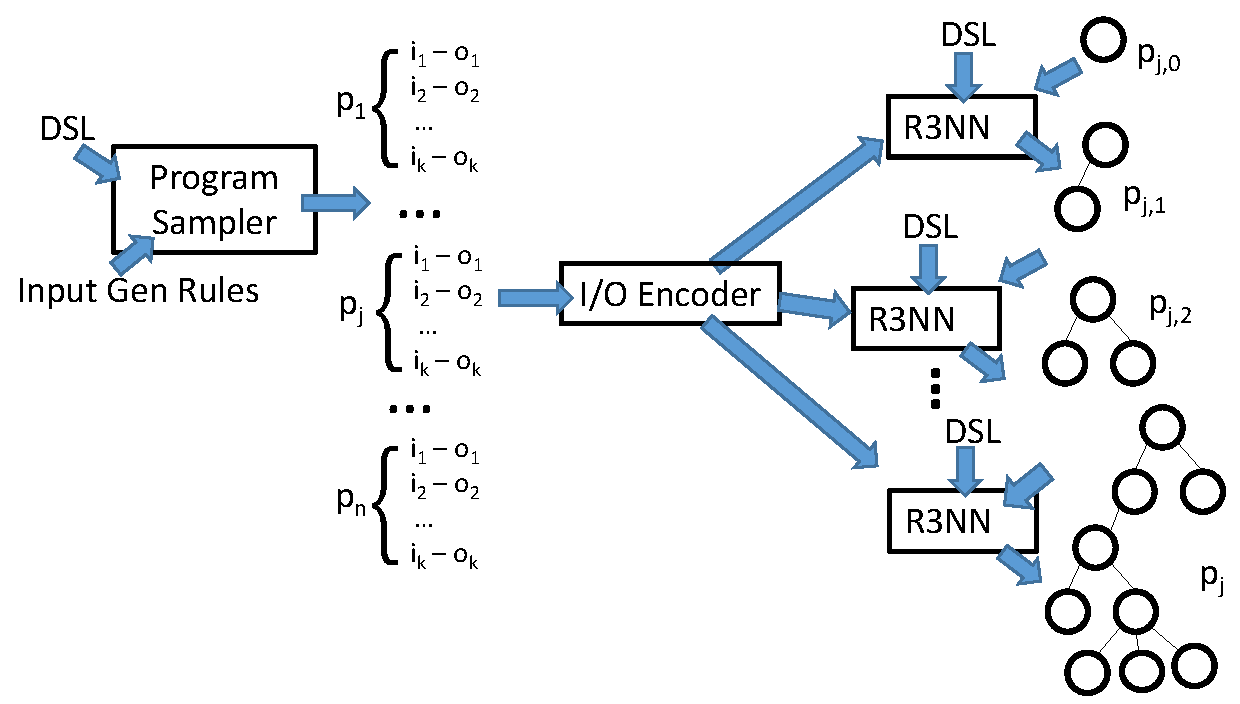
\includegraphics[scale=0.3]{figures/nsps_training.pdf}
        \end{minipage}
        &
        \begin{minipage}{0.5\linewidth}
            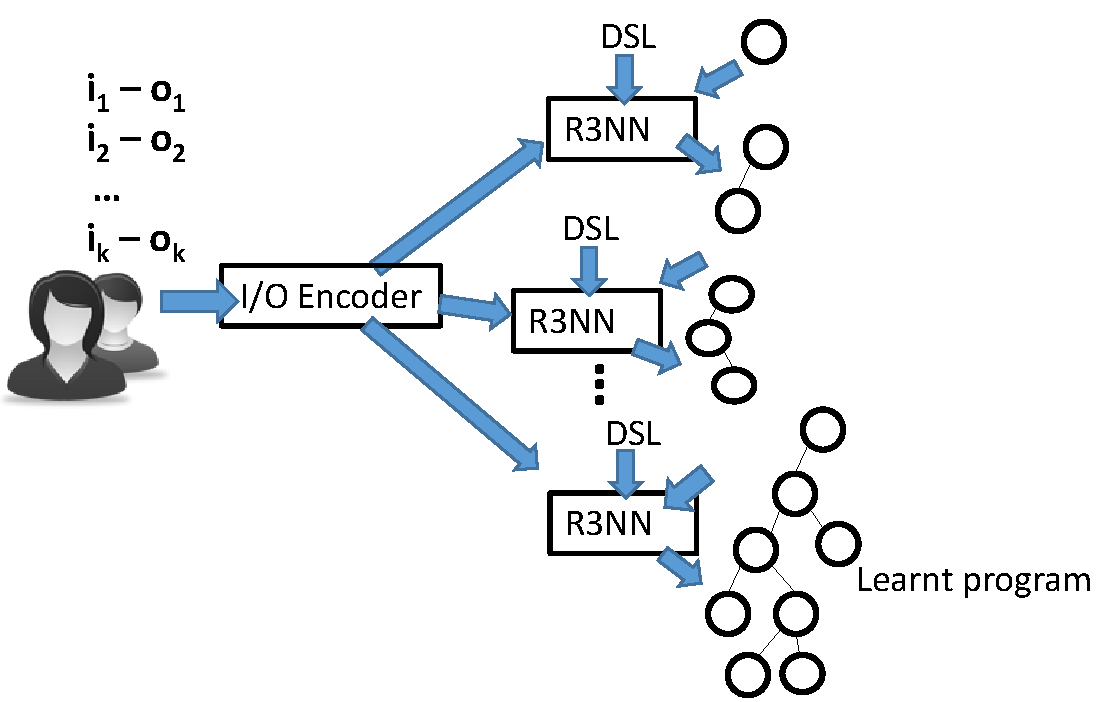
\includegraphics[scale=0.3]{figures/nsps_test.pdf}
        \end{minipage}
        \\
        (a) Training Phase & (b) Test Phase
    \end{tabular}
    \caption{overview of the Neuro-Symbolic Program Synthesis model, taken from \citep{nsps}}
    \label{nsps}
\end{figure*}

\citet{nsps} try out different example encoders,
each embedding into a continuous space a one-hot representation of the input or output strings of their domain,
although we have simply stuck with their simple LSTM baseline.
% i.e. for a vocabulary of `a', `b' and `c', encode `b' as $010$,
% meaning the second option out of three.
% They start out with a simple LSTM baseline,
% but progressing through various versions of a \emph{cross-correlation encoder},
% then introduce different variants based on the \emph{cross-correlation}~\citep{bracewell1986fourier} between inputs and outputs.
% sliding the output and input feature blocks over one another to calculate their \emph{cross-correlation}~\citep{bracewell1986fourier},
% then aggregating these by sum or concatenation,
% % using LSTMs instead of dot products then summing,
% then using two more involved approaches using LSTMs.

The baseline sample encoder processes input/output strings of example pairs
using two separate deep bidirectional LSTM networks,
one for inputs, one for outputs.
For each I/O pair, it then concatenates the topmost hidden representation
at every time step to produce a $4HT$-dimensional feature vector per I/O pair,
where $T$ is the maximum string length for any input or output string,
and $H$ is the topmost LSTM hidden dimension controlling the amount
of features we would like per one-hot encoded characters.
It then concatenates the encoding vectors across all I/O pairs
to get a vector representation of the entire I/O set.~\citep{nsps}

\begin{figure*}[h]
    \begin{tabular}{cc}
        \begin{minipage}{0.45\linewidth}
            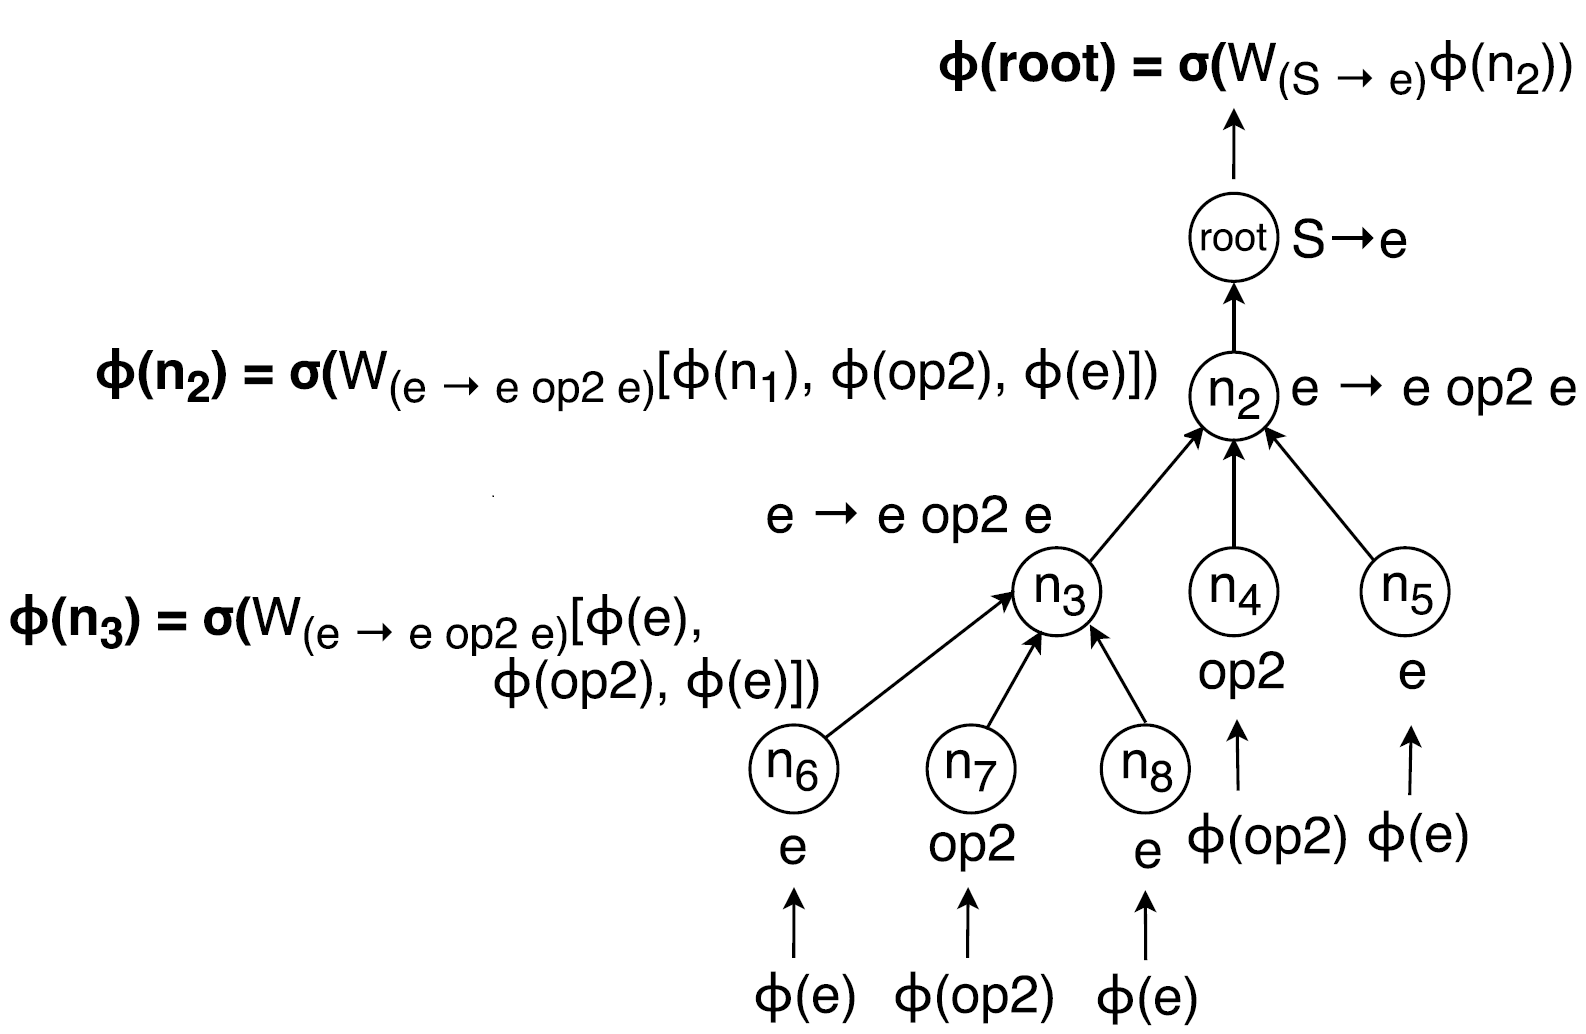
\includegraphics[scale=0.16]{figures/tree2.png}
        \end{minipage}
        &
        \begin{minipage}{0.55\linewidth}
            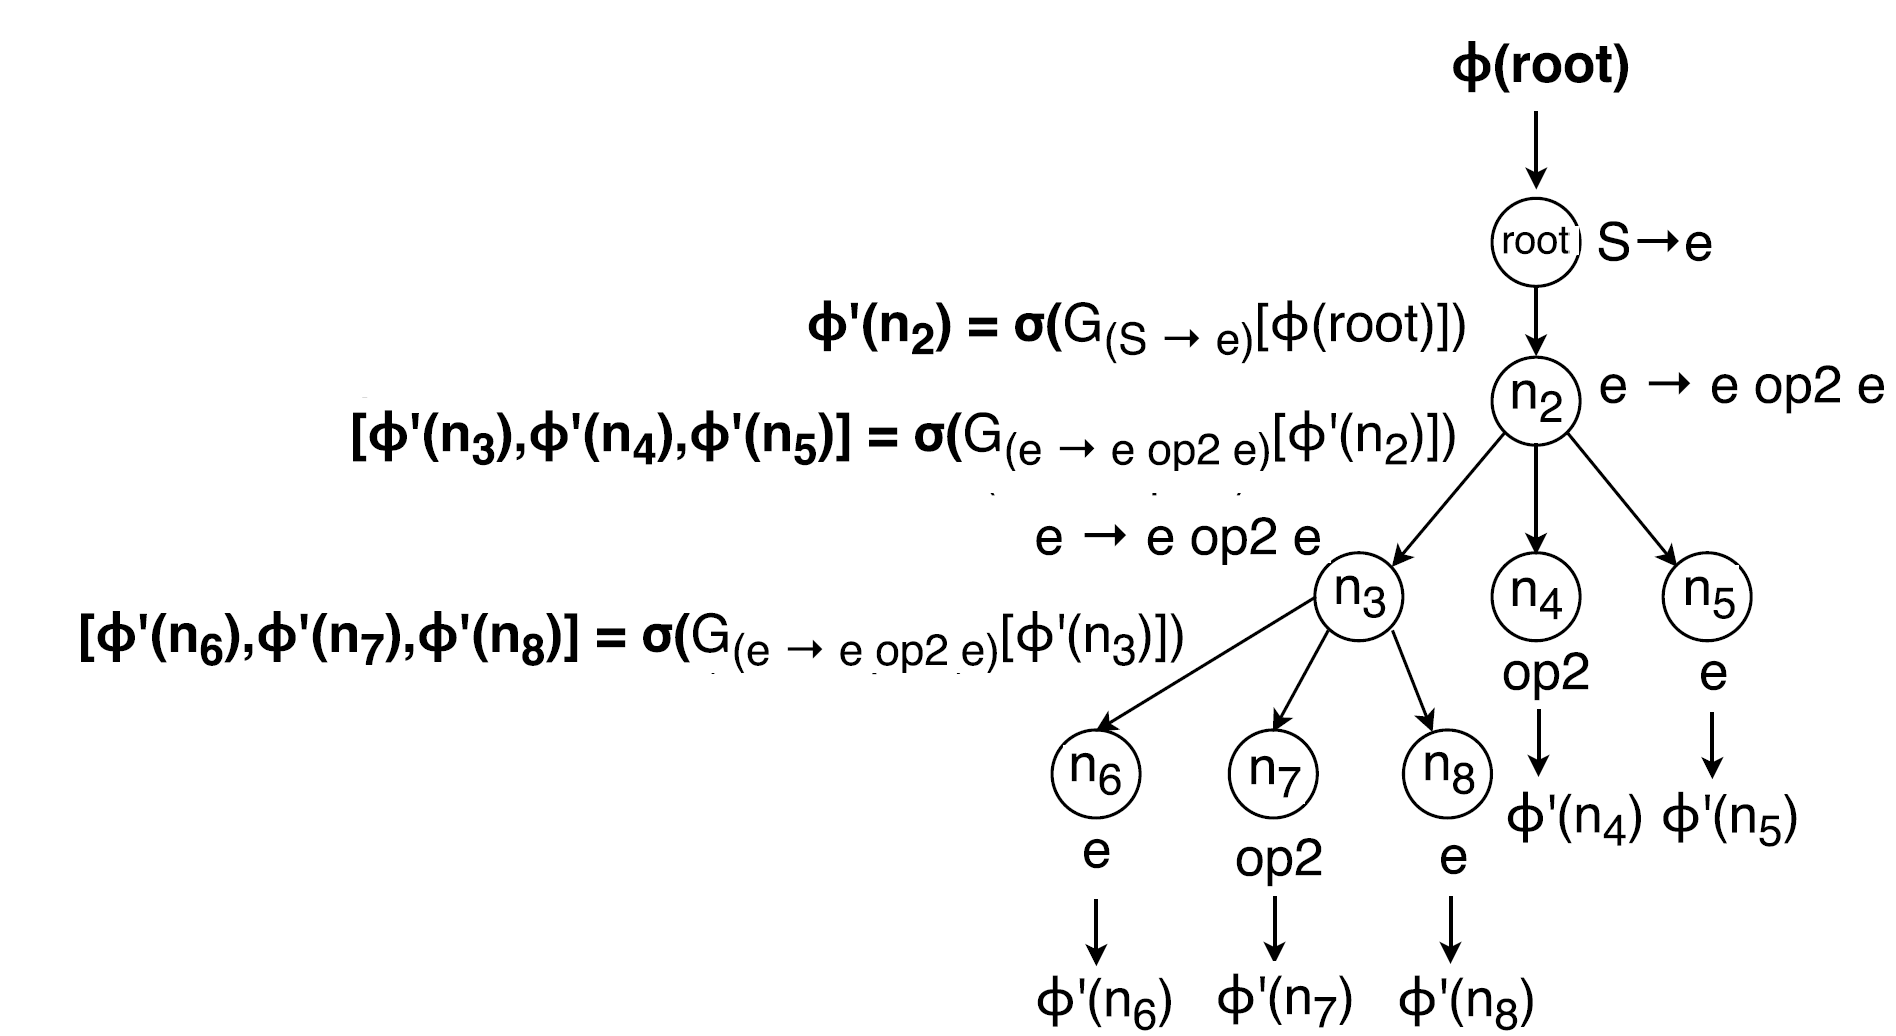
\includegraphics[scale=0.16]{figures/tree3.png}
        \end{minipage}
        \\
        (a) Recursive pass & (b) Reverse-Recursive pass
    \end{tabular}
    \caption{(a) The initial recursive pass of the R3NN. (b) The reverse-recursive pass of the R3NN where the input is the output of the previous recursive pass. Illustrations taken from \citep{nsps}.}
    \label{r3nn}
\end{figure*}

The workings of the R3NN are illustrated in Figure \ref{r3nn}.
The R3NN utilizes two parallel sets of neural networks, $f_r$ and $g_r$,
both consisting of one neural net per grammar production rule $r \in R$.
In the diagram these are denoted by $W(r)$ and $G(r)$, respectively,
with $r$ calculated as production rule $R(n)$ of non-leaf node $n$.
or determined by its symbol $s \in S$ at any leaf $l \in L$,
where $s$ represents an operator in our grammar, calculated by $S(l)$.
These two sets correspond to the R3NN's two passes through an AST (explained below).
Their neural networks use a single layer with hyperbolic tangent activation function (denoted by $\sigma$).

R3NN defines a hyperparameter $M$ indicating the number of features used in their embeddings.
It uses this in an embedded representation $\phi(s) \in \mathbb{R}^M$
for every operator in the DSL (e.g. \verb|+|), which they refer to as \emph{symbols} $s \in S$,
as well as in a representation $\omega(r) \in \mathbb{R}^M$ for every production rule $r \in R$.

The R3NN first makes a \emph{recursive pass} from the embeddings $\phi(l)$
of leaves $l \in L$ of the program tree gradually toward the root node of the partial program,
making for an embedding $\phi(root)$ of the full program so far.
Given a number of child nodes $Q$ of the branch in question
(as dictated by the grammar expansion rule it represents),
this recursive pass goes through neural networks $f_r$ at each branch,
mapping from $Q \cdot M$ to $M$ dimensions,
i.e. from concatenated right-hand side (RHS) vectors to a left-hand side (LHS) vector.

It then performs a \emph{reverse recursive pass} from this root embedding $\phi(root)$,
now passing back to the leaves through $g_r$,
one of a second set of neural networks,
mapping back from $M$ to $Q \cdot M$ dimensions,
i.e. from a LHS vector back to concatenated RHS vectors $\phi'(c)$ for any node $c$.
% which now have their individual embeddings instilled with structural information about the entire program and how they fit into this larger structure.
%
In the event a node $c$ constitutes a non-leaf node $n$,
this process is then repeated, until reaching leaf embeddings $\phi'(l)$.
% Such leaf embeddings $\phi'(l)$ are now different for leaf nodes sharing the same symbol,
% while before these two passes their original embeddings $\phi(l)$ would have been identical.

\citet{nsps} define an \emph{expansion} $e \in E$ as a combination of a hole (non-terminal leaf node) $e.l$ and a grammar production rule $e.r$, together making up for a way we can expand our PPT.
Expansion scores of an expansion $e$ they define as the dot product of their respective embeddings:
$z_e = \phi'(e.l) \cdot \omega(e.r)$.

These scores are then normalized to probabilities using a \emph{softmax} operation.
They find processing leaf embeddings $\phi'(l)$ by a bidirectional LSTM%
~\citep{huang2015bidirectional} before the score calculation helped as well.
To condition R3NN expansion probabilities on the input-output examples specifying desired program behavior in PBE,
they concatenate them to the node features $\phi$ before the recursive pass.

For the test phase they sample 100 programs from their trained model.
They consider the synthesized program to have passed if any of these demonstrate the correct behavior on the input/output.
%
As this is a strongly supervised model,
the loss $J^{(task)}_{PPT}$ predicting one hole-expansion for a task function $task$ given a
partial-program tree $PPT$ is defined as the cross-entropy between our predicted probability matrix
$\mathbf{\hat{P}}_{PPT}$ (over holes $H$ and expansion rules $R$)
versus the golden `probabilities' $\mathbf{P}^{(task)}_{PPT}$ as per the task function we are supervising against.

% If the task function consists of more than a single node, then we will obtain such a loss for every such prediction step (each starting from their own $PPT$).
% Note that the $PPT$ we start from in a prediction step is carried over to inform our next rule expansion.
% Informing our current prediction using previous predictions in such a way makes the model \emph{autoregressive}~\citep{kendall1944autoregressive}.

\section{Methodology} % \label{sec:methodology}

In this section we will briefly discuss our synthesis DSL, then explain our PBE model,
which applies type information to improve synthesis quality in programming by example,
and how it relates to NSPS~\citet{nsps}.
% explain the functional programming synthesis DSL we use with this to exploit its features,
% as well as how we generate datasets in order to obtain training and test sets in our DSL.
%
% To explain the design decisions we made,
% we will go by the synthesizer taxonomy of \citet{gulwani2017program} introduced in Section \ref{sec:litreview}.
% The first two criteria, i.e. constraints on expressions of user intent and search space,
% together give the background needed to understand both our dataset generation method as well as the synthesizer itself.
% We will therefore first explain our design decisions with regard to these,
% then continue to lay out the design of our dataset generation method and synthesizer.

To test our hypothesis we generate a programming-by-example (PBE) dataset in the functional programming domain
based on a subset of the \emph{lambda calculus}~\citep{church1940formulation}
allowing variables and function application though not function definition,
implemented by simply using a subset of Haskell as our synthesis DSL.

Viewing a program as a composition of function applications guarantees us that any complete type-checking program from the root,
filtered to the right output type, will yield us output of the desired type,
helping us reduce our synthesis search space to a sensible subset,
devoid of e.g. programs containing variable definitions that end up never being used.
This guarantees that, rather than just branching out,
our search will focus on finding acceptable solutions.

Our synthesis approach itself is agnostic to the set of operators used,
allowing for relatively straight-forward experimentation with different sets of operators.
% Adding new operators simply involves generating a new dataset, then retraining the model.
% We will further expand on our operator set in Section \ref{sec:experiment}.
%
An example showing what different components of our dataset items might look like may be found in Figure \ref{fig:datasample}.
%
\begin{figure*}
    \begin{tabular}{|l|l|} \hline
        \textbf{task function} & \verb|let just = Just; compose = (.) in compose just unzip| \\ \hline
        \textbf{type instance parameter input types} & \verb|[(Int, Char)]| \\ \hline
        \textbf{type instance output type} & \verb|Maybe ([Int], [Char])| \\ \hline
        \textbf{input expression} & \verb|([((17), '0'), ((20), '2')])| \\ \hline
        \textbf{output expression} & \verb|Right (Just ([17, 20], "02"))| \\ \hline
    \end{tabular}
    \caption{A task function instance from our dataset with a corresponding sample input/output pair.}
    \label{fig:datasample}
\end{figure*}
%
We \emph{unroll} any function applications in our grammar, such that given a binary function operator \verb|and| and a an operator \verb|false| taking no arguments it might look as follows:

\begin{verbatim}
expr = "(and ", expr, " ", expr, ")";
expr = "(and ", expr, ")";
expr = "and";
expr = "false";
\end{verbatim}

\subsection{Typed Neuro-Symbolic Program Synthesis}

% \subsubsection{Our adaptation of neuro-symbolic program synthesis} \label{sec:ournsps}

For conditioning programs we use a (bidirectional) LSTM.
We also use \citet{nsps}'s bidirectional LSTM processing global leaf representations right before score calculation.
As a place for input-output conditioning we use \emph{pre-conditioning}
(adding embedded input-output examples before the recursive pass).
As in the original paper, we sample 100 programs on evaluation.
We aggregate losses over an epoch by taking their mean.

% \subsubsection{Functional program domain} \label{sec:fp}

% % Aside from the grammar we have described in Section \ref{sec:grammar},
% Translating \citet{nsps}'s synthesizer from its original \emph{FlashFill}~\citep{prose} domain to our domain of \emph{functional programs},
% we made the following adjustments:

% \begin{itemize}
    % \item
    While the input-output samples used by \citet{nsps} were all \emph{strings},
    in our functional domain these could essentially comprise arbitrary expressions.
    % While ideally a synthesizer would respect the tree-like structure of such expressions as ASTs,
    Our naive approach has been to simply perform \emph{sample serialization} here,
    taking string versions of our actual input/output expressions,
    then \emph{one-hot encode} the strings' characters as \citet{nsps} did using their string samples.

    % We sample a fixed number of i/o pairs per task function instance during dataset generation as the R3NN's conditioning LSTM requires a fixed amount.

% \subsubsection{Types} \label{sec:typednsps}

We will now explain how we augment the NSPS model to incorporate type info.
% We also refer back to NSPS's hyperparameters $T$, $H$ and $M$ here,
% where $T$ indicates the maximum string length for any input or output string,
% $H$ controls the amount of features per one-hot encoded characters,
% $M$ indicates the number of features the \emph{R3NN} uses in its embeddings,
% $\omega(r)$ the production rule embeddings,
% and $\phi(s)$ the symbol embeddings.
%
Consistent with how we embed expressions, we similarly serialize types to strings,
then one-hot encode their characters as we do for input/output expressions.
To get the most out of our types, we will want to provide them for:
\begin{itemize}
    \item inputs and outputs,
    which we simply incorporate as additional features in \citet{nsps}'s
    \emph{example encoder} as explained in Section \ref{sec:nsps},
    concatenating their one-hot embeddings to those of the input/output pairs before passing them through the input/output LSTMs,
    % increasing the amount of features per sample under their baseline
    % LSTM encoder by another $4HT$
    making for a total of $8HT$ features per sample;

    \item expressions from expansion rules $r$; % based on our operators from Section \ref{sec:grammar};
    for these we may calculate types statically upfront,
    then embed these to obtain $M \cdot T$ features per expansion rule $r \in R$,
    and during R3NN prediction concatenate these features to the existing
    representation $\omega(r) \in \mathbb{R}^M$,
    yielding $\omega'(r) \in \mathbb{R}^{M \cdot (T+1)}$.

    \item (hole) AST nodes $c$ in any PPT.
    % A proper attempt here would be based on type inference across the program.
    %
    % For the sake of simplicity, however, we will settle for simply using the hole's
    % parent branch node to obtain its parameter type without type variables filled out,
    % i.e. a \emph{local} type that has yet to take into account some of the type information available elsewhere in the PPT.
    %
    During prediction in the R3NN, we embed these types by an LSTM into $M \cdot T$ features per hole type.
    As with rule embeddings, we then concatenate these with the original $M$ hole node features,
    once concatenated together, yielding $\phi''(l) \in \mathbb{R}^{M \cdot (T+1)}$.

\end{itemize}

Having obtained our respective rule and hole embeddings expanded to $M \cdot (T+1)$ from the original $M$ features,
we would then proceed to calculate the scores from these enhanced embeddings using the same calculations as before,
simply swapping out the embeddings to their enhanced versions,
i.e. going from $z_e = \phi'(e.l) \cdot \omega(e.r)$ to $z_e = \phi''(e.l) \cdot \omega'(e.r)$.

% The basic idea here is simple:
% on the type level we may provide information not only about how outputs correlate to inputs,
% but may also provide info about how our expansion rules may match up to particular holes in our program.
% Using this extra information should improve our search,
% as per our research hypothesis. % \#1.
% % \ref{hyp:types}.

% \pagebreak

\section{Experiment} \label{sec:experiment}

To perform our experiment, we first find an appropriate learning rate on our vanilla implementation of NSPS,
otherwise taking the hyperparameter values described in Section \ref{sec:hpar}.
% 
We will then evaluate on our task to evaluate a few different models;
our vanilla implementation of \citet{nsps}'s NSPS model,
our type-based additions described in \ref{sec:typednsps},
as well as an enlarged version of the vanilla model for fair comparison.
To reduce variance, we run each model to convergence using $4$ different seeds.
For final evaluation, we provide a uniform random synthesizer as a reference baseline as well.

% \subsection{Benchmark task} \label{sec:task}

We pick our own set of types and operators to generate a dataset as described in Section \ref{sec:datagen}.
For this purpose we have picked a limited set of operators widely applicable over the types used.
Types used include \verb|Char|, \verb|Int|, \verb|Maybe|, \verb|List|, \verb|(,)|, and \verb|Either|.
%
We have picked the following set of operators for our chosen types:
\verb|0|, % "zero"  -- did I need this in like foldr?
\verb|Just|, % "just"
\verb|maybe|, % "maybe"
% List
\verb|(:)|, % "(:)"
\verb|length|, % "length"
% (,)
\verb|(,)|, % "(,)"
\verb|zip|, % "zip"
\verb|unzip|, % "unzip"
% Enum
\verb|toEnum|, % "toEnum"  -- from Int to any of our scalars
\verb|fromEnum|, % "fromEnum"  -- from any of our scalars to Int
% Foldable
\verb|foldMap|, % "foldMap"
\verb|elem|, % "elem"
% Traversable
\verb|sequenceA|, % "sequenceA"
\verb|sequence|, % "sequence"
% Functor
\verb|fmap|, % "fmap"
% Monoid
\verb|mempty|, % "mempty"  -- may replace [], Nothing, HashMap.empty, Set.empty
% Semigroup
\verb|(<>)|, % "(<>)"
%
and \verb|(.)|.

% \pagebreak

\section{Result} \label{sec:result}

Having added our type-level supervision during training, we expect synthesis success rates to rise
compared to the baseline algorithm.
This demonstrates that the findings from traditional program synthesis methods are relevant also in the field of neural program synthesis.

Any results here are trained on our dataset spanning programs of up to 3 nodes,
during training evaluated by sampling 100 programs from the synthesizer for any task function instance.

\begin{figure*}[h]
    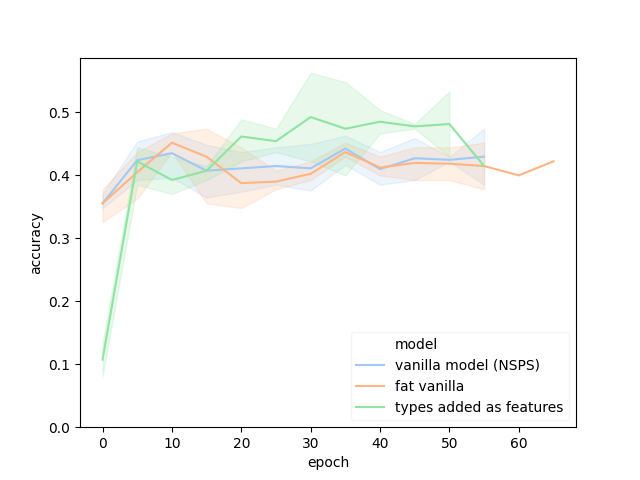
\includegraphics[scale=0.6]{figures/experiments.png}
    \caption{
        Prediction accuracy over 100 samples across training epochs for our different model variants,
        trained on our dataset of programs of up to 3 nodes.
    }
    \label{fig:accuracy}
\end{figure*}

Accuracy results over training on our validation set can be found in Figure \ref{fig:accuracy},
while accuracy on the test set for the fully trained models may be found in Figure \ref{fig:finalacc}.
We see that the simpler vanilla NSPS model is both more limited in variance while also learning to a more limited extent before converging.

Our first observation here is that the task has turned out relatively challenging,
with accuracy for the baseline model increasing only somewhat beyond its initial random accuracy.
Furthermore, most of the gains in accuracy for the baseline model are attained over the initial 10 epochs of training.
We feel these issues may be explained largely from the limited size of our dataset.

We additionally trained an enlarged version of this baseline model,
doubling the sample encoder output dimension parameter $H$ from $32$ to $64$,
giving it a similar amount of expressiveness as our typed model as a reference.
To our surprise however, this model
fared little better than the baseline, again likely stemming
from generalization issues related to the size of our dataset.

Our `typed' NSPS model however,
keeping $H$ at $32$ but allotting that same amount for types,
starts from sub-random accuracies, yet ends up able to learn more,
after $20$ epochs out-performing both our baseline and enlarged models,
indicating it is in fact worthwhile to distribute features between input/output pairs and types.

\begin{figure*}
    \begin{tabular}{|l|c|c|c|c|c|c|c|c|c|c|} \hline
        & \multicolumn{5}{|c|}{ \textbf{evaluated @ 20 samples} } & \multicolumn{5}{|c|}{ \textbf{evaluated @ 100 samples} } \\ \hline
        & \multicolumn{2}{|c|}{ \textbf{accuracy} } & \multicolumn{3}{|c|}{ \textbf{acc mean @ x nodes} } & \multicolumn{2}{|c|}{ \textbf{accuracy} } & \multicolumn{3}{|c|}{ \textbf{acc mean @ x nodes} } \\ \hline
        \textbf{experiment} & \textbf{mean} & \textbf{var} & \textbf{1} & \textbf{2} & \textbf{3} & \textbf{mean} & \textbf{var} & \textbf{1} & \textbf{2} & \textbf{3} \\ \hline
        \textbf{vanilla NSPS} & 0.13 & 0.000 & 0.27 & 0.13 & 0.11 & 0.37 & 0.000 & 0.77 & 0.36 & 0.30 \\ \hline
        \textbf{large} & 0.12 & 0.001 & 0.30 & 0.12 & 0.09 & 0.38 & 0.002 & 0.73 & 0.38 & 0.30 \\ \hline
        \textbf{typed} & \textbf{0.22} & 0.002 & \textbf{0.55} & \textbf{0.24} & \textbf{0.12} & \textbf{0.48} & 0.003 & 0.77 & \textbf{0.55} & \textbf{0.34} \\ \hline
        \textbf{uniform random} & 0.14 & 0.000 & 0.43 & 0.11 & 0.11 & 0.33 & 0.000 & \textbf{0.84} & 0.25 & 0.31 \\ \hline
    \end{tabular}
\caption{
    Summary of final prediction accuracy on our test set over different models after training (4 seeds each),
    for each selecting the best-performing epoch as per validation accuracy i.e. before overfit.
    Results are separated by evaluation on 20 vs. 100 samples,
    and metrics include mean accuracy, variance of accuracy,
    as well as mean accuracy separated by programs of a given number of nodes. Bolded cells indicate the best accuracy in a given category.
}
\label{fig:finalacc}
\end{figure*}

We additionally attempted to look into whether we could find a correlation between this
advantage gained by incorporating type information (as seen in Figure \ref{fig:ttest}) with the number of nodes in a program.
However, the data we managed to gather was insufficient to demonstrate such a correlation.

Specifically, our task turned out hard,
with none of the models significantly out-performing a random synthesizer
on the task functions of 3 nodes.
On the 1-node task functions at 100 samples,
similarly none of the models outperformed the random synthesizer's 84\% accuracy,
although at 20 samples the typed model out-performed it at 55\% vs. 43\%.
This means that most of the learning success for these models has been on the 2-node task functions,
particularly for the typed model, achieving over double the random accuracy for either 20 or 100 samples.

Unfortunately for our purposes, performing best on the 2-node programs
means we cannot presently distinguish any clear correlation between
task function node size and advantage from type information.
As such, we would love to see similar experiments scaled up to larger datasets including higher node sizes.

In order to verify the statistical significance of our proposed model variant,
we have performed an independent two-sample t-test comparing the accuracy across our models
(as evaluated on 20 samples per task function instance),
results for which may be found in Figure \ref{fig:ttest}.

Whereas we similarly compared such differences for accuracy as evaluated on 100 samples,
we found the outcome for 20 samples to more clearly demonstrate the difference between models.
Under 4 seeds each our typed model turns out to have only p=1.0\%
to stem from the same distribution as our baseline model,
indicating the improvement in performance is statistically significant.

\begin{figure*}
    \begin{tabular}{|l|c|c|c|c|c|c|} \hline
        \textbf{p-values}
        & \textbf{vanilla} & \textbf{large} & \textbf{types} & \textbf{uniform} \\ \hline
        \textbf{vanilla} & 1.000 & 0.859 & 0.010 & 0.013 \\ \hline
        \textbf{large} & 0.859 & 1.000 & 0.024 & 0.065 \\ \hline
        \textbf{types} & 0.010 & 0.024 & 1.000 & 0.001 \\ \hline
        \textbf{uniform} & 0.013 & 0.065 & 0.001 & 1.000 \\ \hline
    \end{tabular}
    \caption{P-values for different model combinations under the independent two-sample t-test comparing accuracy as evaluated on 100 samples per task function instance.}
    \label{fig:ttest}
\end{figure*}

% \pagebreak

\section{Discussion} % \label{sec:discussion}

\subsection{Design limitations}

\begin{itemize}
    \item
    We settled for \citet{nsps}'s \emph{baseline LSTM encoder} rather than its more complex \emph{cross-correlation} encoders.

    \item
    We disregard any programs exceeding a limit of 3 nodes, both on dataset generation as well as on synthesis.

    \item
    Our present implementation unfortunately still defers full type inference in favor of \emph{local types} based on our unrolled grammar,
    so it cannot fill in further type variables based on information elsewhere in the program tree.

\end{itemize}

\subsection{Topics for future research}

As neural synthesis methods aimed at programming by example in the functional
programming domain is a broad topic encompassing a variety of design decisions,
we have had to leave some questions unanswered.
% We will give an overview in this section of some of the questions raised during our design process specifically.

% \begin{itemize}

    % compile RL
    % \item 
    While we have focused on types as features here,
    %  and compilation for masking purposes
    after each synthesis step,
    % in languages featuring \emph{typed holes},
    % a type of dummy variable for which the compiler can tell the appropriate type
    % as well as providing suggestions of what in-scope variables might fit said hole,
    we might also \emph{pre-compile} even partial programs such as to provide the synthesizer with immediate feedback on whether a program type-checks;
    as with types, we similarly hypothesize neural program synthesis methods can benefit from using compilation checks as additional features.
    %
    However, this would require a \emph{weakly supervised} neural synthesizer,
    i.e. using \emph{reinforcement learning},
    whereas our present synthesizer is based on the simpler \emph{strongly supervised} setup.
    As such, this was unfortunately out of scope for our current paper.

    % operators and type advantage
    % \item 
    While we have looked into the added value of types as features,
    this gives rise to an additional question:
    what kind of operators are most conducive to benefiting from type info?
    While we have briefly conjectured this to involve having few yet generically applicable operators,
    this question has fallen out of scope for our paper,
    and remains a question for future research.

    % % unrolling
    % % \item 
    % As we touched upon in Section \ref{sec:grammar},
    % the merits of our \emph{unrolled grammar} approach are still up for empirical evaluation.
    % As our present dataset allowed us to settle for this approach,
    % we decided to regard this question as out of scope for our present paper.

% \end{itemize}

\subsection{Conclusion}

% Programming by example has traditionally seen a split between formal versus neural approaches,
% meaning programming types had yet to be used in neural program synthesis.
We presented a way to incorporate programming types into a neural program synthesis approach for programming by example.
We generated a dataset in the functional programming context,
and demonstrated type information to improve synthesis accuracy even given a comparable number of parameters.
Finally, we suggest a number of topics of interest for future research in type-driven neural programming by example.

% \pagebreak

% % \bibliographystyle{acm}
% % \bibliographystyle{plainnat}
% \bibliographystyle{iclr2021_conference}
% \bibliography{references}

% \pagebreak

% \appendix

% \section{Hyperparameters} \label{sec:hpar}

% \subsection{Hyperparameters used for dataset generation} \label{sec:gen-params}

% % The hyperparameters we have used in our dataset generation have been as follows:
% % \begin{description}
% %     \item[crashOnError (default false, for experiment specify true)] when specified just crash on error while calculating function outputs. otherwise perform an additional typecheck (slower).
% %     \item[nestLimit (1)] max number of levels of nesting for generated types. high values make for big logs while debugging...
% %     \item[maxInstances (5)] max number of instances to generate for any type containing type variables. may get less after deduplicating type instances.
% %     \item[numInputs (10)] max number of inputs to generate. may get less after nub filters out duplicates.%
% %     ~\footnote{This setting directly follows \citet{nsps}.}
% %     \item[maxHoles (3)] the maximum number of holes to allow in a generated expression
% %     \item[numMin (-20)] the minimum value for numbers to generate
% %     \item[numMax (20)] the maximum value for numbers to generate
% %     \item[charMin ('0')] the minimum value for characters to generate
% %     \item[charMax ('9')] the maximum value for characters to generate%
% %     ~\footnote{
% %         The decision to restrict characters to digits was made with the intent to let their characters overlap
% %         with those of digits for the purpose of helping reduce characters used in the encoder,
% %         in turn reducing the size of its one-hot embedding.
% %         This arbitrary constraint serves no other purpose than to constrain required compute.
% %     } 
% %     \item[listMin (0)] the minimum number of elements to generate for list types
% %     \item[listMax (5)] the maximum number of elements to generate for list types
% %     % figure out a sensible split. NSPS mentions training/test tho not validation.
% %     % We sample a subset of only 1000 training programs from the 5 million program set to report the training results in the tables. The test sets also consist of 1000 programs.
% %     \item[splits] train (0.35) / validation (0.35) / test (0.3)
% %     \item[maxDataset (10000)] the maximum number of programs we will consider for use in our dataset (before further filtering)
% % \end{description}

% In this section we will describe the hyperparameter values we have used in our dataset generation.

% % \item[crashOnError (default false, for experiment specify true)] when specified just crash on error while calculating function outputs. otherwise perform an additional typecheck (slower).
% % nestLimit
% We generate types to substitute into \emph{type variables} using a maximum of only \emph{one} level of nesting,
% i.e. allowing type \emph{list of booleans} though not type \emph{list of lists of booleans}.

% % maxInstances
% For any parameter type containing type variables used in task functions,
% we generate a maximum of $5$ type \emph{instances}, before deduplication.
% % numInputs
% Whereas \citet{nsps} generated $10$ inputs for each task function,
% we instead generate up to $10$ for each \emph{type instance} of a task function, before deduplicating.

% % maxHoles
% While they limited functions to a maximum of $13$ operations,
% we instead limit ours to a maximum of $3$,
% given that our current operator set is considerably bigger than those of their \emph{FlashFill} domain.

% % numMin, numMax
% Numbers that we generate, all of them integers,
% we limit to the range from $-20$ to $20$.
% % charMin, charMax
% For characters we stick to the range of digits, i.e. from `0' to `9',
% a decision made with the intent to let their characters overlap
% with those of digits for the purpose of helping reduce characters used in the encoder,
% in turn reducing the size of its one-hot embedding.
% This arbitrary constraint serves no other purpose than to constrain required compute.

% % listMin, listMax
% Data structures such as \emph{string}, \emph{list}, \emph{set}, and \emph{hashmap},
% we each generate using lengths in the range from $0$ to $5$.
% Of these, \emph{sets} might further deduplicate down,
% as this structure only holds unique items.

% % splits
% % NSPS mentions training/test tho not validation: We sample a subset of only 1000 training programs from the 5 million program set to report the training results in the tables. The test sets also consist of 1000 programs.
% Our dataset we split into training, validation and test sets
% using a ratio of $35\%$, $35\%$, and $30\%$, respectively.
% % maxDataset
% As \citep{nsps} we sample $1,000$ training programs from the total function space.

% % fixed in our synthesizer
% \subsection{Hyperparameters in our synthesizer} % \label{sec:synth-params}

% In this section we will describe the hyperparameter values we have during the training and evaluation of our synthesizers.

% % \begin{description}
% %     \item[NumLayers (3)] the number of hidden layers used in the LSTMs in our sample encoder
% %     (for both input and output), for our type encoders (for rule expansions and holes),
% %     as well as for sample conditioning and scoring in \citet{nsps}'s \emph{R3NN}.
% %     % \item[seed] 
% %     \item[numEpochs (1000)] the maximum number of epochs to train for.
% %     % while these batch parameters were inspired by NSPS's, mine apply to batches of input/output samples, while theirs pertain to batches of task functions.
% %     \item[encoderBatch (8)] the encoder batch size i.e. number of samples to process in one go.
% %     \item[r3nnBatch (8)] the R3NN batch size i.e. number of i/o samples to sample per invocation
% %     \item[bestOf (100)] Number of functions to sample from the model for each latent function and set of input/output examples that we test on, determining success based on the best from this sample.%
% %     ~\footnote{This setting directly follows \citet{nsps}.}
% %     \item[evalFreq (5)] the number of epochs for which to run on train set before evaluating on the validation set again.
% %     \item[learningRate (0.001)] initial learning rate used in ML optimizer.
% %     \item[checkWindow (default 1, for experiment specify 2)] the window of evaluations to check over to verify convergence.
% %     \item[convergenceThreshold (0.000001)] the minimum loss increment we consider as indicating convergence.
% %     \item[learningDecay (5)] by how much to divide the learning rate when accuracy decreases.
% %     % \item[maxHoles] the maximum number of holes to allow in a generated expression
% %     \item[evalRounds] the maximum number of rounds to evaluate for during hyperparameter optimization. by default all configurations are evaluated.
% %     \item[maskBad] when specified, compile any possible hole fill to mask out any predictions for non-compiling expressions (present implementation for this is slow but this could be improved).
% %     \item[useTypes] supervise synthesis using rule/hole types as additional features.
% %     %
% %     % \item[dropoutRate (0.0)] the \emph{dropout rate}~\citep{baldi2014dropout} used in any LSTMs.%
% %     % % for which we search over values [\num{0.0}, \num{3.125e-2}, \num{6.25e-2}, \num{0.125}, \num{0.25}, \num{0.5}];
% %     % ~\footnote{We saw no mention of this in \citet{nsps}'s original implementation, so figured this would be deemed optional.}
% %     % \item[regularization (0.0)] the L2 regularization rate~\citep{zhang2018three}, for which we search over values [\num{0.0}, \num{1.0e-4}, \num{1.0e-3}, \num{1.0e-2}, \num{0.1}],
% %     \item[M (32)] the number of features used in our symbol and expansion rule embeddings as per \citet{nsps}'s \emph{R3NN}.
% %     % for which we search over values [\num{8}, \num{16}, \num{32}, \num{64}, \num{128}],
% %     \item[H (32)] the number of features used per input or output per LSTM direction as per \citet{nsps}'s \emph{baseline LSTM encoder}.
% %     % for which we search over values [\num{8}, \num{16}, \num{32}, \num{64}, \num{128}],
% %     \item[hidden0 (16), hidden1 (16)] the number of hidden units for the 
% %     (respectively first and second) 
% %     hidden layers used in the \emph{MLP}s of \citet{nsps}'s \emph{R3NN}'s \emph{recursive} and \emph{reverse-recursive} passes.
% %     % for which we search over values [\num{4}, \num{8}, \num{16}, \num{32}, \num{64}].
% % \end{description}

% % NumLayers
% We use $3$ layers in our LSTMs, which are present in our sample encoder
% (for both input and output), our type encoders (for rule expansions and holes),
% as well as for sample conditioning and scoring in our \emph{R3NN}.
% % The neural cells in the \emph{recursive} and \emph{reverse-recursive}
% % passes of the \emph{R3NN} are fixed to using only a single layer with hyperbolic tangent activation.
% We do allow bias terms although the original paper did not show these in their formulas.
% % seed
% % numEpochs
% We train for a maximum of $1,000$ epochs.

% % encoderBatch
% Our \emph{encoders} process items (either input-output samples or types) using a batch size of $8$.
% % r3nnBatch
% Our \emph{R3NN} must use a fixed number of embedded input-output pairs on the basis of its LSTM used for conditioning,
% and as such we have fixed this to use samples of $8$ embedded input-output pairs.
% % while these batch parameters were inspired by NSPS's, mine apply to batches of input/output samples, while theirs pertain to batches of task functions.
% % bestOf

% As \citet{nsps}, for synthesizer evaluation we sample $100$ functions from the model for each task function,
% determining success based on the best from this sample,
% i.e. considering the synthesis a success if any of these pass our PBE task, exhibiting the desired behavior.

% % evalFreq
% We evaluate performance on our validation set once after every $5$ epochs of training.
% % % learningRate
% % For our Adam optimizer we use an \emph{initial learning rate} of \num{1e-3},
% % % learningDecay
% % subsequently further decreased by a factor of $5$ whenever accuracy is found to decrease during evaluation.
% % checkWindow
% During evaluation we similarly check for convergence based on the loss,
% averaging over windows of $2$ evaluations,
% i.e. stop training if the validation loss over the past two evaluations has increased from the two before.

% % convergenceThreshold
% % ditching this cuz honestly it doesn't do anything
% % considering as an indication of convergence only loss increments of at least \num{1e-6}.

% % maxHoles
% We arbitrarily limit synthesized functions to the same complexity limit of $6$ operators as used during generation of task functions.
% % % evalRounds
% % While we allow a maximum number of hyperparameter configurations to evaluate during hyperparameter optimization, by default all configurations are evaluated.
% % maskBad
% % \item[maskBad] when specified, compile any possible hole fill to mask out any predictions for non-compiling expressions (present implementation for this is slow but this could be improved).
% % useTypes
% % \item[useTypes] supervise synthesis using rule/hole types as additional features.

% % dropoutRate
% % We use a \emph{dropout rate}~\citep{baldi2014dropout} in any LSTMs of $0\%$.%
% % % ~\footnote{We saw no mention of this in \citet{nsps}'s original implementation, so figured this would be deemed optional.}
% % regularization
% % We use an \emph{L2 regularization rate}~\citep{zhang2018three} of $0.0$.
% % M
% We allow $32$ features in our symbol and expansion rule embeddings, i.e. $M$ in \citet{nsps}'s \emph{R3NN}.
% % H
% We allow $32$ features per input or output per LSTM direction, i.e. $H$ in \citet{nsps}'s \emph{sample encoder}.
% % % hidden0/hidden1
% % Finally, we use $16$ hidden units in both hidden layers of the \emph{MLP}s,
% % used in the \emph{recursive} and \emph{reverse-recursive} passes of \citet{nsps}'s \emph{R3NN}.

% We clip gradients to stay within a range from $-1$ to $1$.

% % \subsection{Hyperparameters optimized in a search} \label{sec:hparopt}

% % Hyperparameters we \emph{search} over, rather than fixed up-front,
% % have been picked based on the question of whether we expected them to have a `sweet spot' in terms of optimum value,
% % rather than being an obvious case of `higher is better';
% % these include:
% % \begin{itemize}
% %     \item dropout rate~\citep{baldi2014dropout},
% %     for which we search over values [\num{0.0}, \num{3.125e-2}, \num{6.25e-2}, \num{0.125}, \num{0.25}, \num{0.5}];
% %     % \item L2 regularization rate~\citep{zhang2018three}, for which we search over values [\num{0.0}, \num{1.0e-4}, \num{1.0e-3}, \num{1.0e-2}, \num{0.1}],
% %     \item the number of features \emph{M} used in our symbol and expansion rule embeddings as per \citet{nsps}'s \emph{R3NN},
% %     for which we search over values [\num{8}, \num{16}, \num{32}, \num{64}, \num{128}],
% %     \item the number of features \emph{H} used per input or output per LSTM direction as per their \emph{baseline LSTM encoder},
% %     for which we search over values [\num{8}, \num{16}, \num{32}, \num{64}, \num{128}],
% %     \item the number of hidden units for the 
% %     % first and second 
% %     hidden layers used in the \emph{recursive} and \emph{reverse-recursive} passes of their \emph{R3NN},
% %     for which we search over values [\num{4}, \num{8}, \num{16}, \num{32}, \num{64}].
% % \end{itemize}

% % This search is performed by a genetic algorithm~\citep{koza1994genetic},
% % used a 20\% \emph{mutation} rate,
% % an 80\% \emph{cross-over} rate,
% % a \emph{population} size fixed to the square root of the total number of hyper-parameter configurations (rounded up),
% % and the \emph{4th root} of the total number of hyper-parameter configurations (again rounded up)
% % used as the maximum number of \emph{generations} and as the number of \emph{best entities} to keep track of.

% % learningRate
% The learning rate for our Adam optimizer we search over
% by a grid search using our vanilla NSPS model, considering
% values of \num{1e-2}, \num{1e-3}, \num{1e-4}, and \num{1e-5}.
% Of these, we settle on a learning rate of \num{1e-2}.

% \section{Miscellaneous experiments}

% Aside from our main experiment, we also tried a few other configurations for which we had not managed to obtain conclusive results.

% \subsection{Type filter}

% The first of these was the idea to combine a synthesizer with a compiler check to filter out any non-compiling programs.
% While the downside to this would be that the synthesizer would be made dependent on this extra compiler check,
% incurring a run-time penalty during synthesis, linear in the number of expansion rules provided,
% the advantage to such a setup would be that the synthesizer would no longer need to learn to disregard non-compiling programs itself,
% reducing synthesis to a ranking problem of the compiling (partial) candidate programs.
% % 
% % \paragraph{Type filter} \label{sec:filter}
% % 
% % However, we may also handle this type info outside of the neural level:
% % one may just restrict their search to those AST nodes allowed
% % for the present hole as dictated by the grammar and types,
% % as per our research hypothesis \#2.
% % % \ref{hyp:filter}
% We achieve this by simply masking the predicted scores of uncompiling programs in our NSPS implementation
% (before calculating actual probabilities by softmax) to have no probability, i.e. $p(e)=0.0$.

% While we failed to obtain any significant improvement over the baseline model using this setup,
% this result may well have related to our implementation.
% We presently used the \verb|hint| Haskell library as our interpreter for type-checks,
% which unfortunately yielded false positive compiler errors for types containing ambiguous type variables,
% such as \verb|show undefined|, which the Haskell compiler would resolve to type \emph{string},
% whereas the \verb|hint| library would complain that the \verb|undefined|
% argument would prevent resolving \verb|show|'s type variable.
% %~\citep{hintambiguous}

% As this counter-factual signal would prevent this synthesizer from correctly synthesizing the affected programs,
% the fact that it nevertheless performed on par with our baseline algorithm suggests this approach does in fact have potential.
% While we might have addressed this flaw in our implementation by switching
% from this interpreter library to using Haskell's compiler API directly,
% due to time constraints this unfortunately fell out of scope for this thesis.

% \subsection{Picking holes}

% Although the topic of which hole to fill was not directly touched upon in \citet{nsps},
% our baseline implementation had the synthesizer deterministically fill the first hole
% (under any given order --- we used left-to-right).
% Nevertheless, we did also wonder what the effect might be if we would allow filling any hole.

% During training, we would then opt to randomly pick a hole to try and fill.
% On evaluation, we would then look at the confidence scores for any hole expansions across holes,
% sampling from this full matrix rather than just the vector slice corresponding to the first hole.
% This allows the synthesizer to take into account the relative confidence of expansions for different holes,
% enabling it to forego holes involving more uncertainty in favor of those it feels more confident about,
% which may in turn provide additional information that may then reduce ambiguity for the remaining holes.%
% ~\footnote{
%     An additional advantage of this would be it could more uniformly explore various partial program trees across synthesis steps.
%     That said, uniform exploration there isn't necessarily the ideal situation ---
%     one might for example imagine using weights to prioritize situations our synthesizer is less confident about.
% }

% Unfortunately, we obtained inconsistent results on this model versus our baselines across different experiment attempts,
% originally getting the expected improvement, although in our final implementation we had not managed to reproduce this improvement.
% We had to leave further analysis of these inconsistent results out of scope due to time constraints,
% and as such feel hard-pressed to make definitive statements on the effectiveness of this approach.
% Nevertheless, we consider this to be a topic of interest in AST-based neural program synthesis.


% \pagebreak

% \section{Acknowledgements} % \label{sec:acknowledgements}

% First of all, I would like to thank my supervisor Emile van Krieken,
% who has actively supported me with his broader knowledge on
% program synthesis and AI whenever my own familiarity failed me.

% Furthermore, I would like to thank my assessor Annette ten Teije for approving
% my research direction, despite it falling outside the well-trodden
% path for either artificial intelligence or computer science separately.

% I additionally thank Emilio Parisotto, who helped answer my questions to better understand their neuro-symbolic program synthesis architecture.~\citep{nsps}

% I must also thank my fellow students, discussions with whom helped me
% tremendously throughout this program --- without them,
% I probably wouldn't have made it this far.

% On the implementation, I am further indebted to the HaskTorch team,
% including Austin Huang, Junji Hashimoto, Torsten Scholak, Sam Stites, and Adam Paszke,
% any of whom have not hesitated to advise me when I got stuck
% on technical aspects including HaskTorch, Nix, Haskell, or machine learning.

% I also owe gratitude to my friend Alejandra Ortiz, who was there for me when I needed it.

% Finally, I would like to dedicate this work to Jaques Lagerweij,
% whom I never got to meet.

\end{document}
